\section{Discussion}
\label{discussion}

The methodology of this study converged in a collection of results obtained thought a field research on the importance of maintaining a communication channel between parents and children during distant-parenting situations. In the previous section, the results have been introduced in order to better define the population sampled. The aim of this section, on the other hand, is to construct from such results our own hypothesis on the issue by identifying interesting patterns according to different features of the data (subsection \ref{analysis-results}). Then we will discuss whether such obtained hypothesis could be transposed back to a Chinese context seen for the LBCs issue (\ref{transposability}). Lastly, we will draw an interview protocol we aim to adopt for a future field test in Mainland China that could eventually bring to us the final prove (or disprove) to our hypothesis (\ref{interview-protocol}).

\subsection{Analysis of the results}
\label{analysis-results}

In this first part of the discussion, we aim to get a deeper overview of the obtained results that has been described in the previous section. The goal is to determine whether interesting patterns could be retrieved from the studied population, in accordance with the distant-parenting issue and how this latter is faced by families.

As already mentioned while explaining the content of the survey (see sec. \ref{content-survey}), the literature review proposed substantial differences in the way the father or the mother figure dealt with the distant parenting matter. Unfortunately, as already presented, the data on the parent side is not sufficiently rich to draw such a analysis to determine whether similarities in our test might occur. On the other hand, we might be interested in discovering unknown outlines on the child's side according to features like ages, sex, etc that has not been sufficiently explored yet.

\begin{figure}[h]
    \centering
    \caption{Importance of communication from the parents point according to their child's age during distant-parenting experience}
    \label{fig:plot_1}
    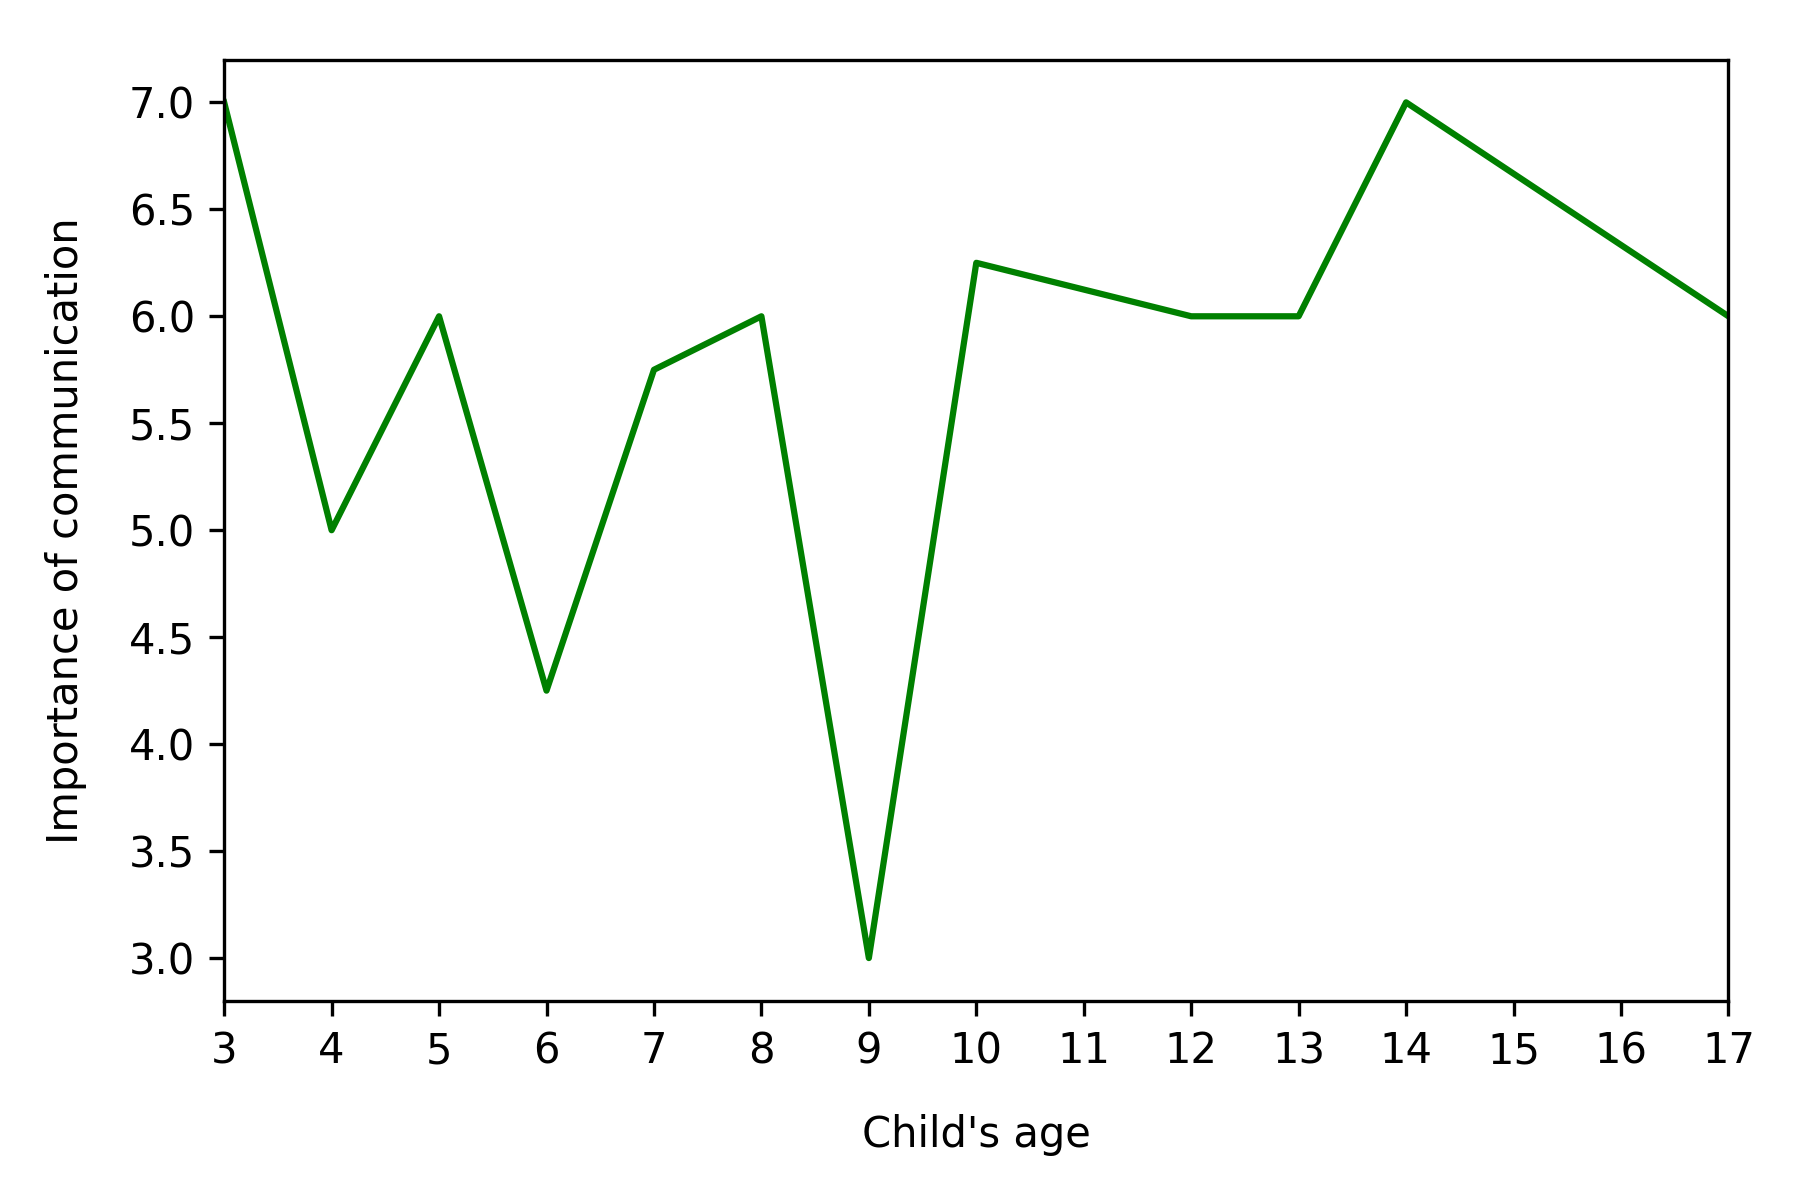
\includegraphics[scale=0.58]{plots/plot_1.png}
\end{figure}

\begin{figure}[h]
    \centering
    \caption{Importance of communication from the children point according to their age during the first time away from home}
    \label{fig:plot_2}
    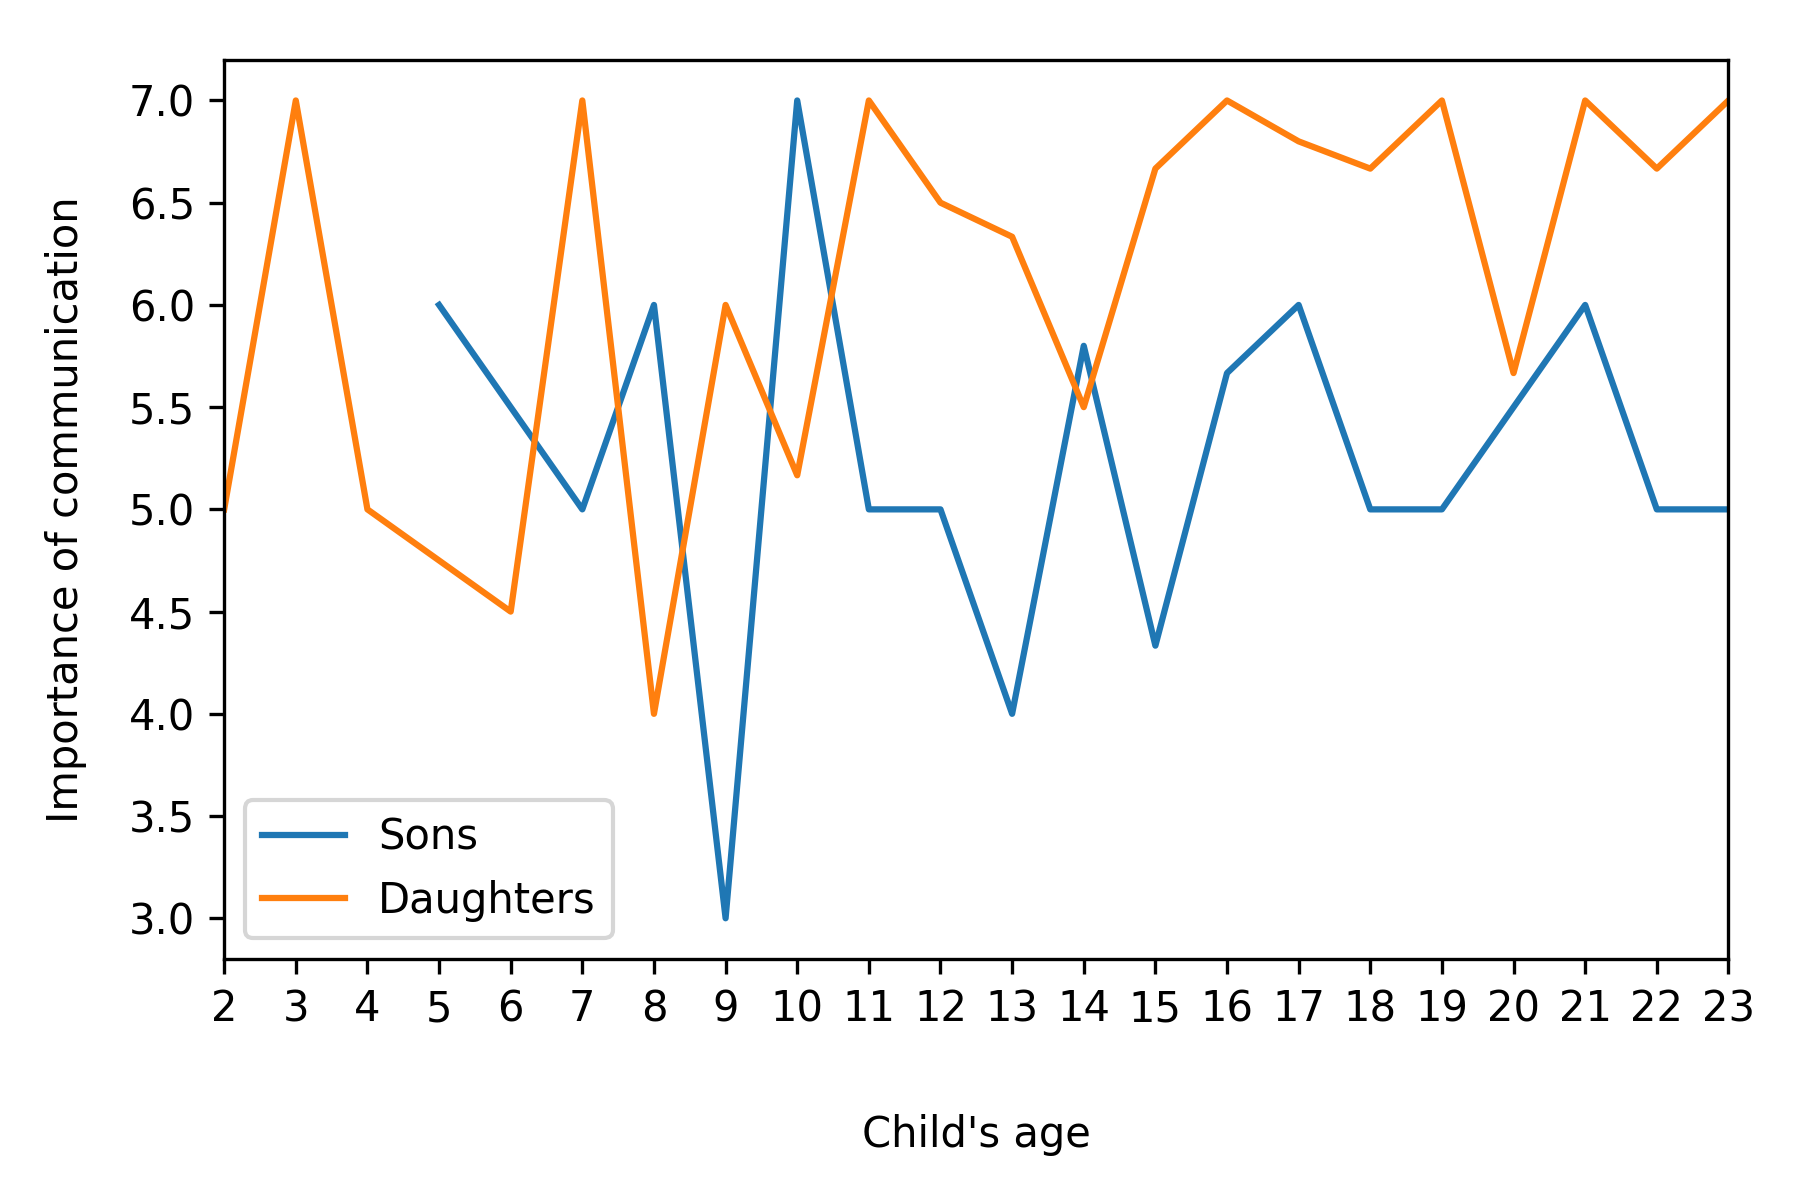
\includegraphics[scale=0.58]{plots/plot_2.png}
\end{figure}

The very first outcome from the data collected is about the feature regarding the importance of communication. We wanted to understand how it was perceived from both the parent and the child side and, specifically, how other factors might modify its trend. The two plots in fig. \ref{fig:plot_1} and fig. \ref{fig:plot_2} illustrate how the usage of communication technologies (ICTs) are perceived from parents and children, according to different child's age during the distant-parenting experience. As already shown in the initial results (see table \ref{tab:stats_children} and table \ref{tab:stats_parents}), the importance is generally perceived extremely high regardless of age differences. Although this latter might seem a trivial consideration, it is useful to keep in mind that such results are strongly related to the context from which they have been extrapolated and might be different in other social conditions and in other cultures such as China. In order to avoid biases of any kind due to triviality in our own perspective, each result need to be considered at this stage to later discuss it in the Chinese context (see sec. <transposability sec ref>).
Moreover, the two plots illustrate already the second consideration we can draw from the results. The trend clearly showcases a strong inclination of female children compared to same aged male peers to give an higher weight to the importance of communication since aged ten years old (fig \ref{fig:plot_2}). Such plot, therefore, suggests a possible exploratory pattern toward different responses according to child's sex and age when being away from home for the very first time. 

The plot presented in fig. \ref{fig:plot_3} tries to relate the frequency of communication between with distant parents-children according to different duration of time children  spent away from their families. The first intuition we had regarding a possible child's sex bias in the data is confirmed by such plot. It generally illustrates an higher tendency for girls to have more frequent communication with their distant families, regardless of the duration of the experience. Girls are more likely to consider a reliable communication channel with their family more important than boys experiencing the same situation.

\begin{figure}[h]
    \centering
    \caption{Frequency of communication distribution according to different distant-family experiences and children's sex}
    \label{fig:plot_3}
    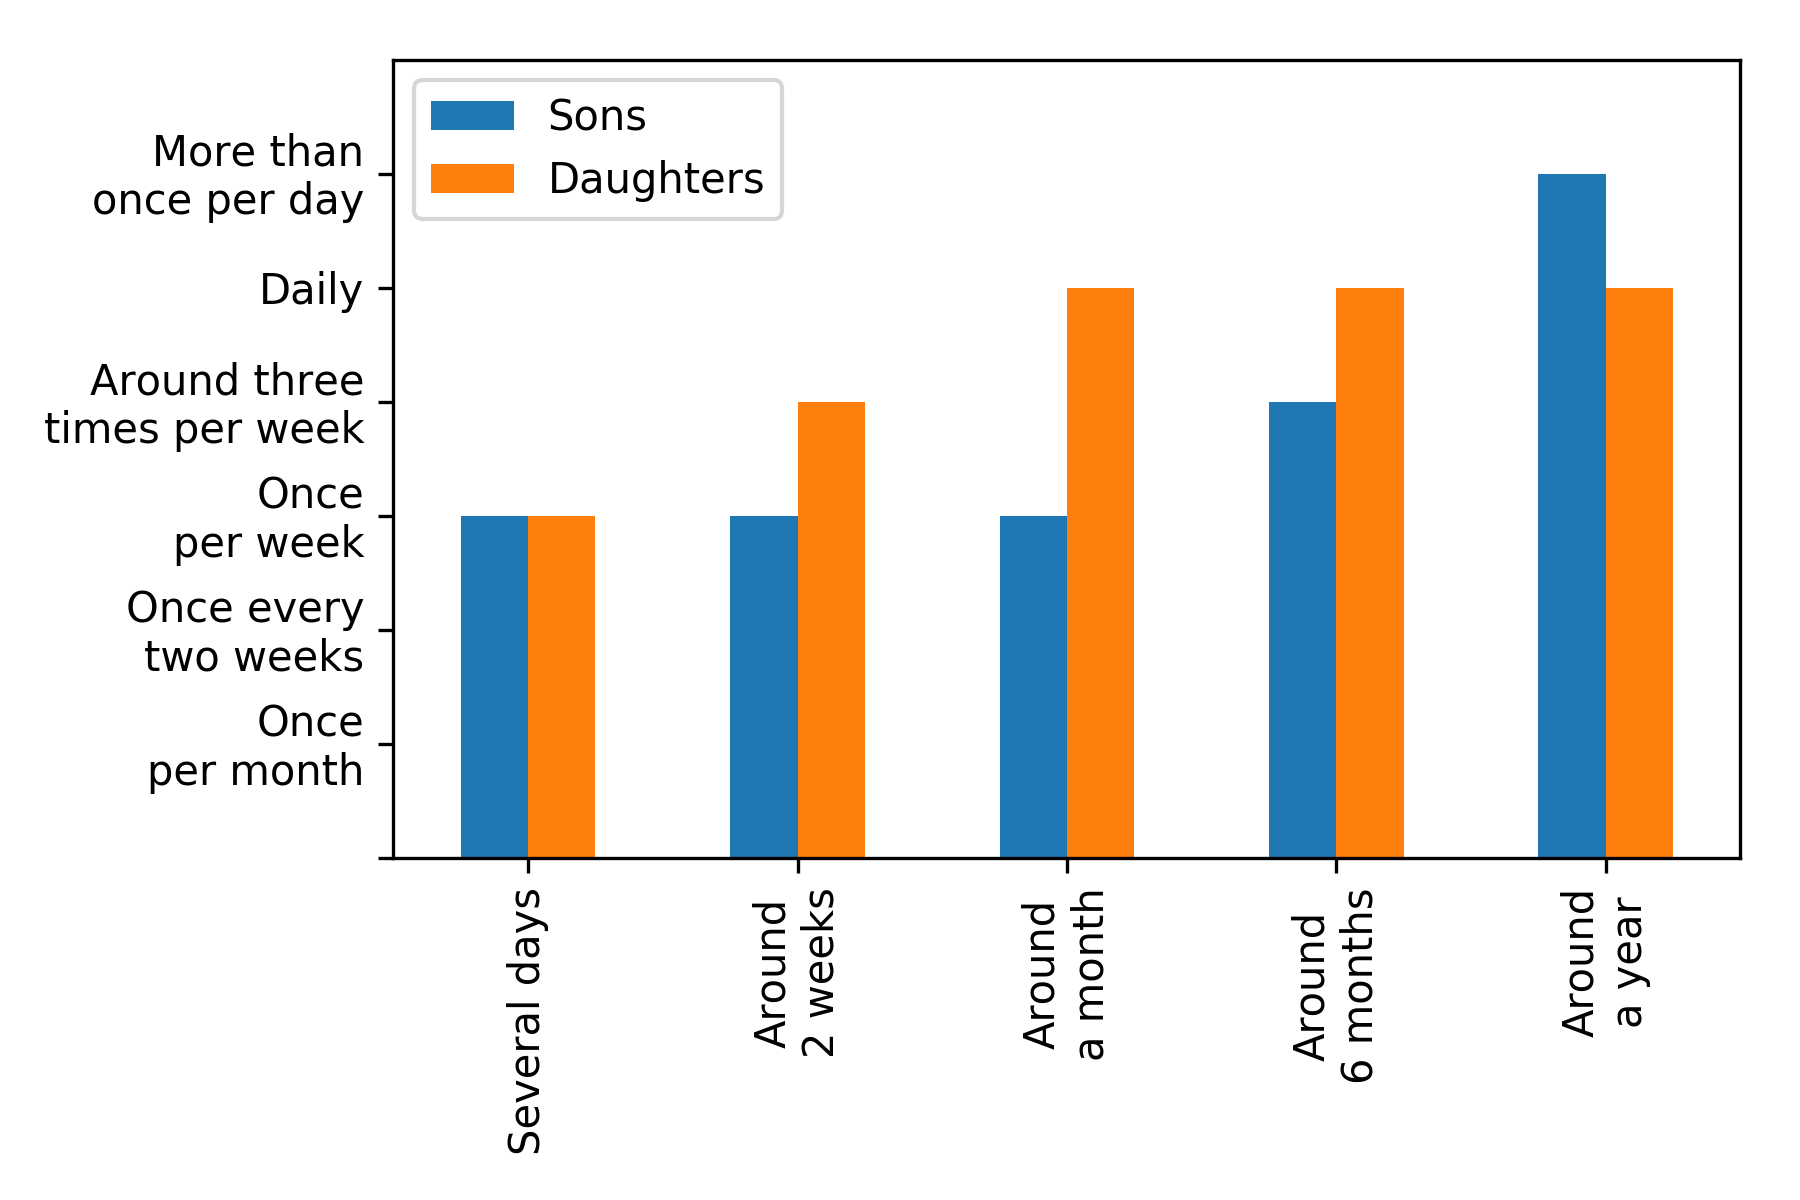
\includegraphics[scale=0.58]{plots/plot_3.png}
\end{figure}

Thanks to the amount of data collected, the exploratory analysis could be conducted on a much higher granularity of distinct representative set. This would allow to better understand what information the data contains and avoid falling in the possible trap of drawing conclusions from outliers. Firstly we decided to project the data according to the duration of the distant-parenting experience for both the parent and children perspective. We aim to determine weather the \textit{"gender bias"} trend could still be appreciated. Plots in fig. \ref{fig:plot_7} and fig. \ref{fig:plot_6} illustrates those findings for the children and parent point of view respectively. Thanks to them we can indistinguishably see the same \textit{"gender bias"} trend, where girls perceive an higher importance of communication when staying away from their family (see fig. \ref{fig:plot_7}). However, it is interesting to compare those results with the parent perspective where this trend is not prominent (see fig. \ref{fig:plot_6}). The importance of communication for parent is generally not affected by the child's sex (nor the duration of the experience neither). Although the data-set collected from the parent side is far from being a reliable sample, results tend to be more homogeneous between  children’s sex (only exception being a short-termed duration of a several days), when compared to the child’s  perspective  illustrated  before. As already discussed previously, in the context from which such data has been collected drawing a conclusion where parents consider equally important a communication channel with their children regardless of their sex might seem trivial. However, every result will be at last evaluated against the Chinese context for which considerable amount of literature exists regarding gender discrepancies, mainly based on the One-Child Policy results of the past decades. Lastly, for the reader's interest, a plot illustrating the same data (from the parent perspective) without any partitioning on features can be found in the appendix \ref{appendix:additional-plots}.

\begin{figure}[h]
    \centering
    \caption{Importance of communication from the children point according to duration of distant-parenting experience}
    \label{fig:plot_7}
    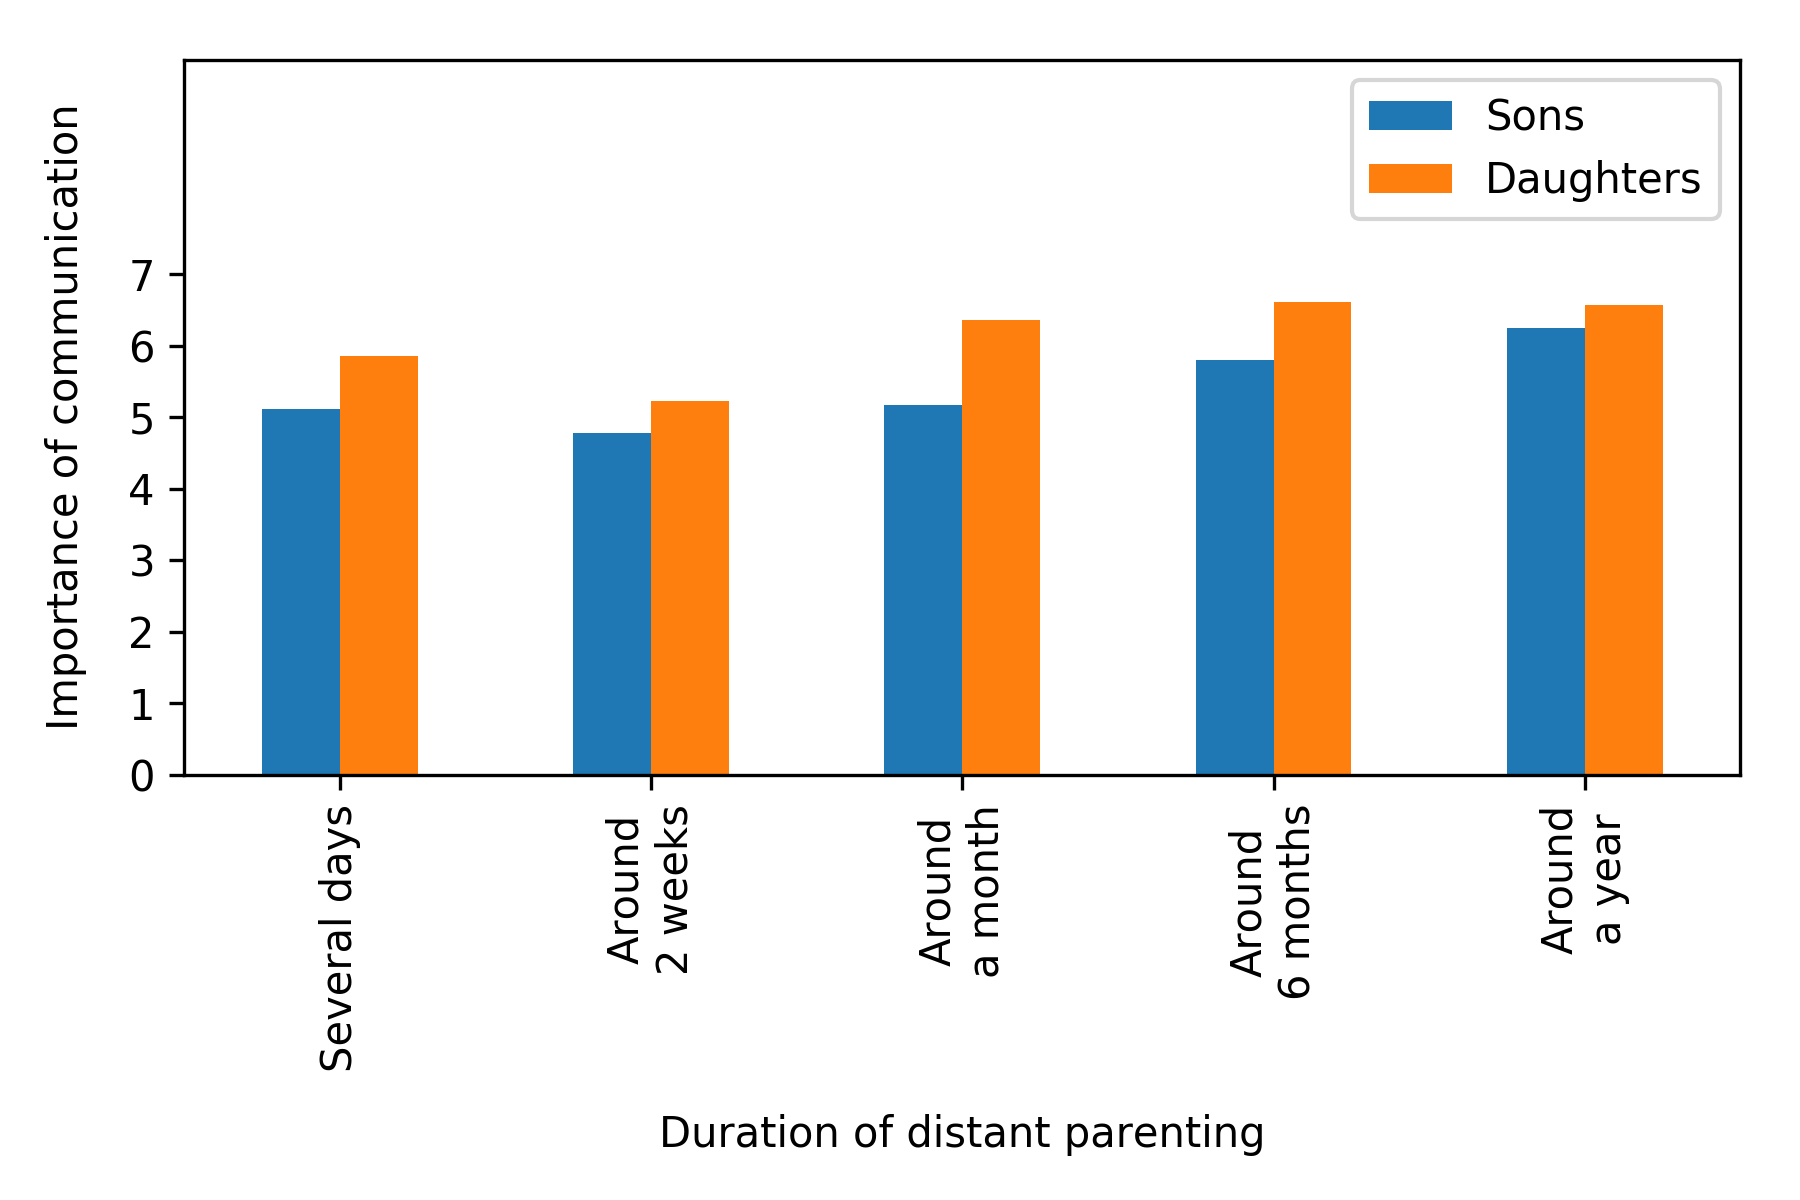
\includegraphics[scale=0.58]{plots/plot_7.png}
\end{figure}

\begin{figure}[h]
    \centering
    \caption{Importance of communication from the parents point according to duration of distant-parenting experience}
    \label{fig:plot_6}
    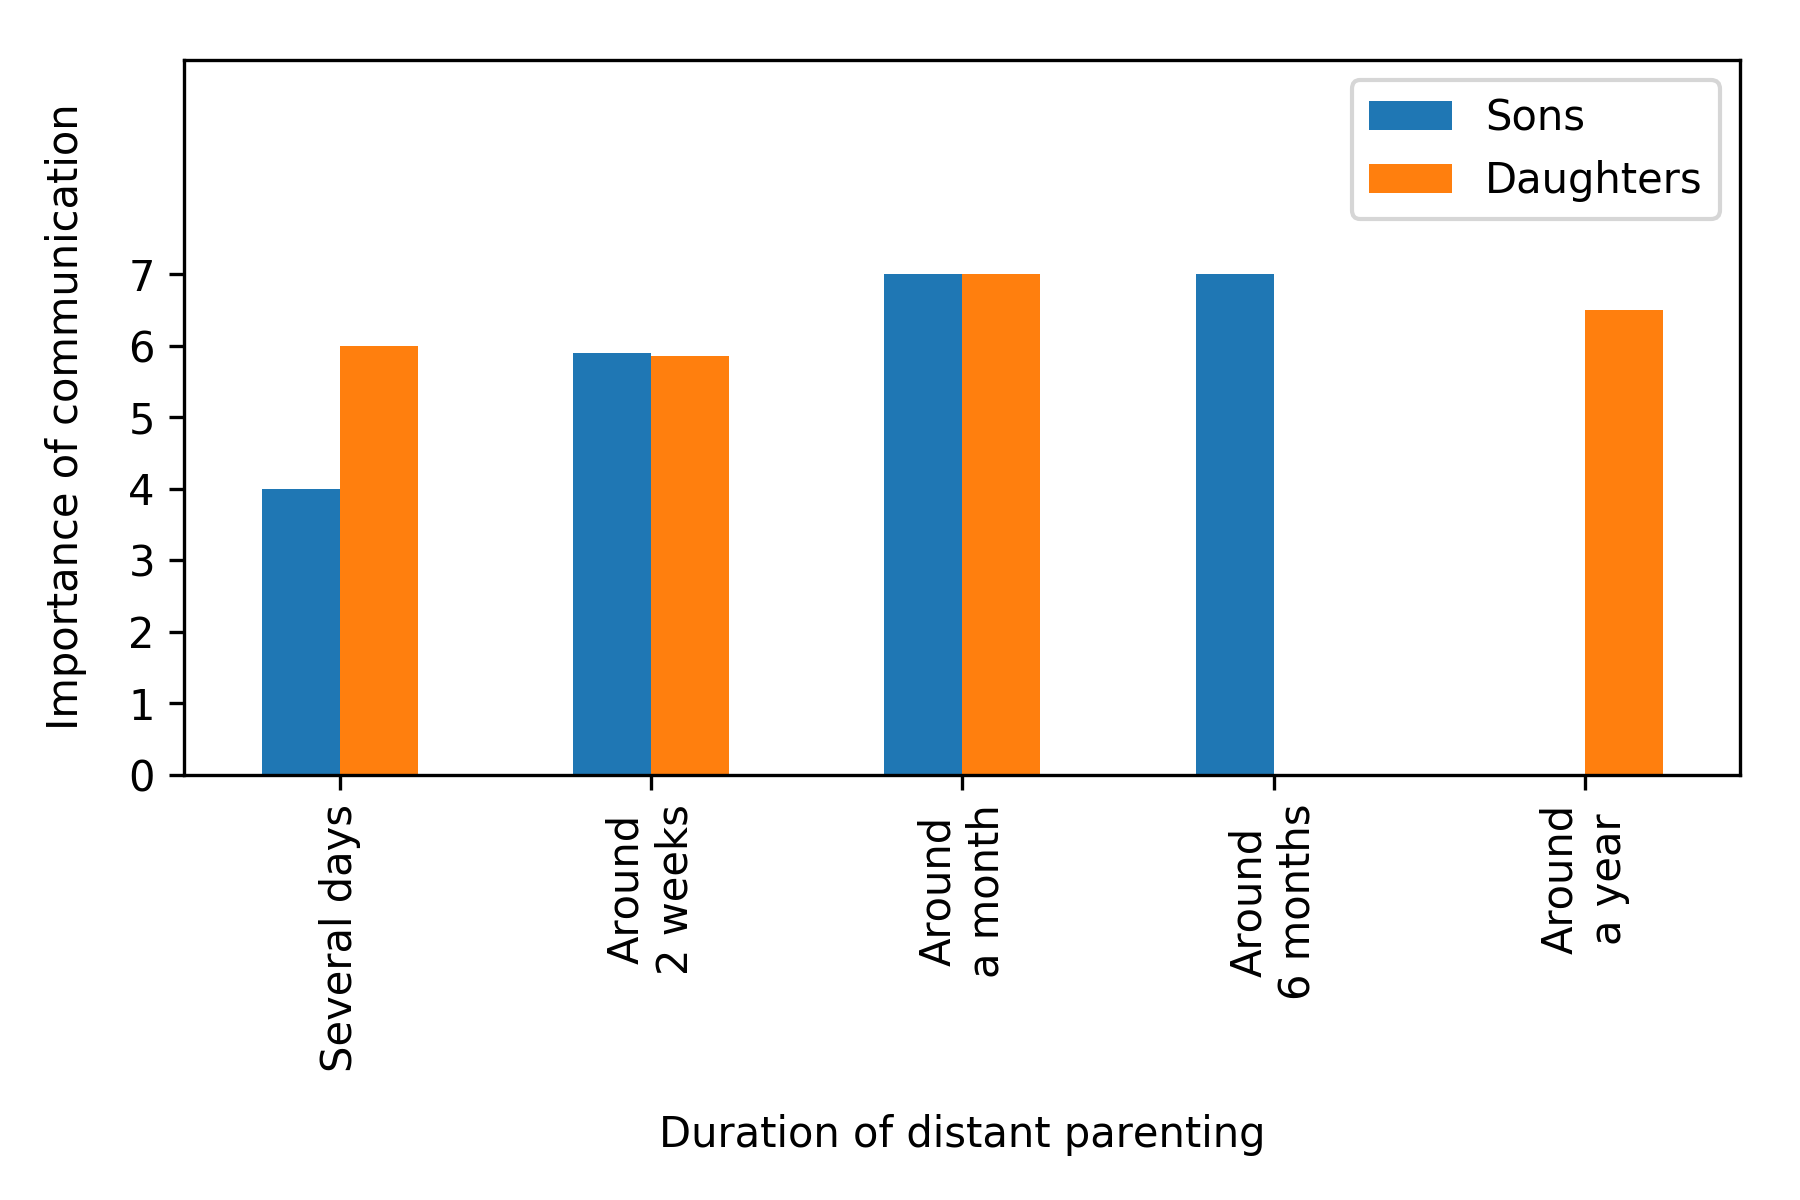
\includegraphics[scale=0.58]{plots/plot_6.png}
\end{figure}
    
The very same analysis for both the parent and children perspective has been conducted again on a \textit{Frequency of communication} factor base. This latter exploratory step in conjunction with the previous computed plots, would help to better define discovered patterns on multiple variables in order to detect variances in the data. The two plots illustrated in fig. \ref{fig:plot_10} and fig. \ref{fig:plot_9} showcases such distributions for the children and parents point of view respectively. As previously proposed, an analysis on the parent data without partitioning, which do not present peculiarities, can be found in the appendix \ref{appendix:additional-plots}. Once again, there is a clear tendency for girls to experience a much higher importance towards communication regardless to how frequent distant families communicate throughout the experience. In short, the bias child's sex showcases with respect to the communication is once again confirmed.  On the other hand, parents tend to not showcase any different behaviour according to their child's sex for this feature as well, confirming the nonexistence of a possible \textit{gender bias} from their point of view. However, it is interesting to underline how both plots (which are modelled around different sample groups, one for children and one for parents) identify a peculiar prominence for boys (or parents with a son) to rate higher the importance of communication whenever the frequency of communication hits the "every other week" point. In order to draw solid conclusions about such peculiarity an higher sampled population would be required to not mistake outliers for patterns.  

\begin{figure}[h]
    \centering
    \caption{Importance of communication from the children point according to the frequency of communication during the distant-parenting experience}
    \label{fig:plot_10}
    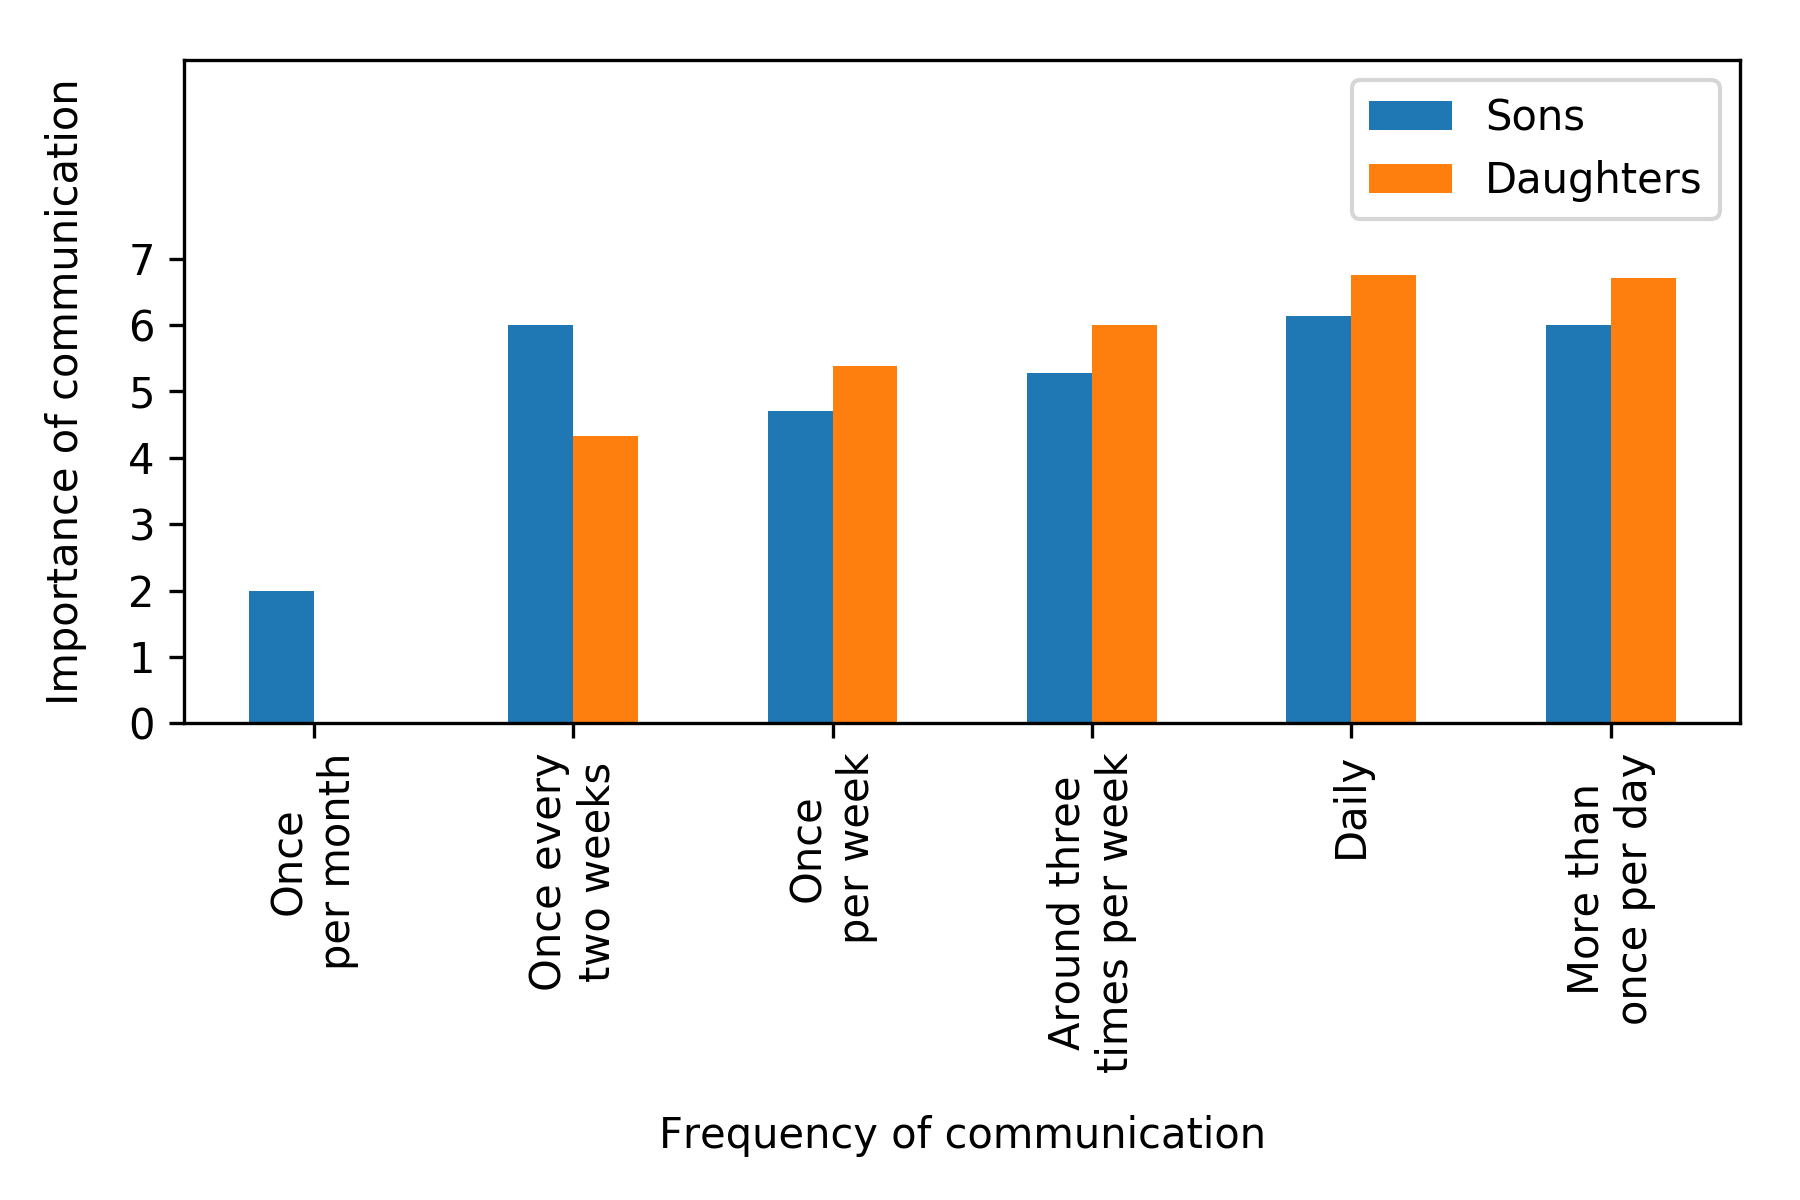
\includegraphics[scale=0.58]{plots/plot_10.png}
\end{figure}

\begin{figure}[h]
    \centering
    \caption{Importance of communication from the children point according to the frequency of communication during the first time away from home}
    \label{fig:plot_9}
    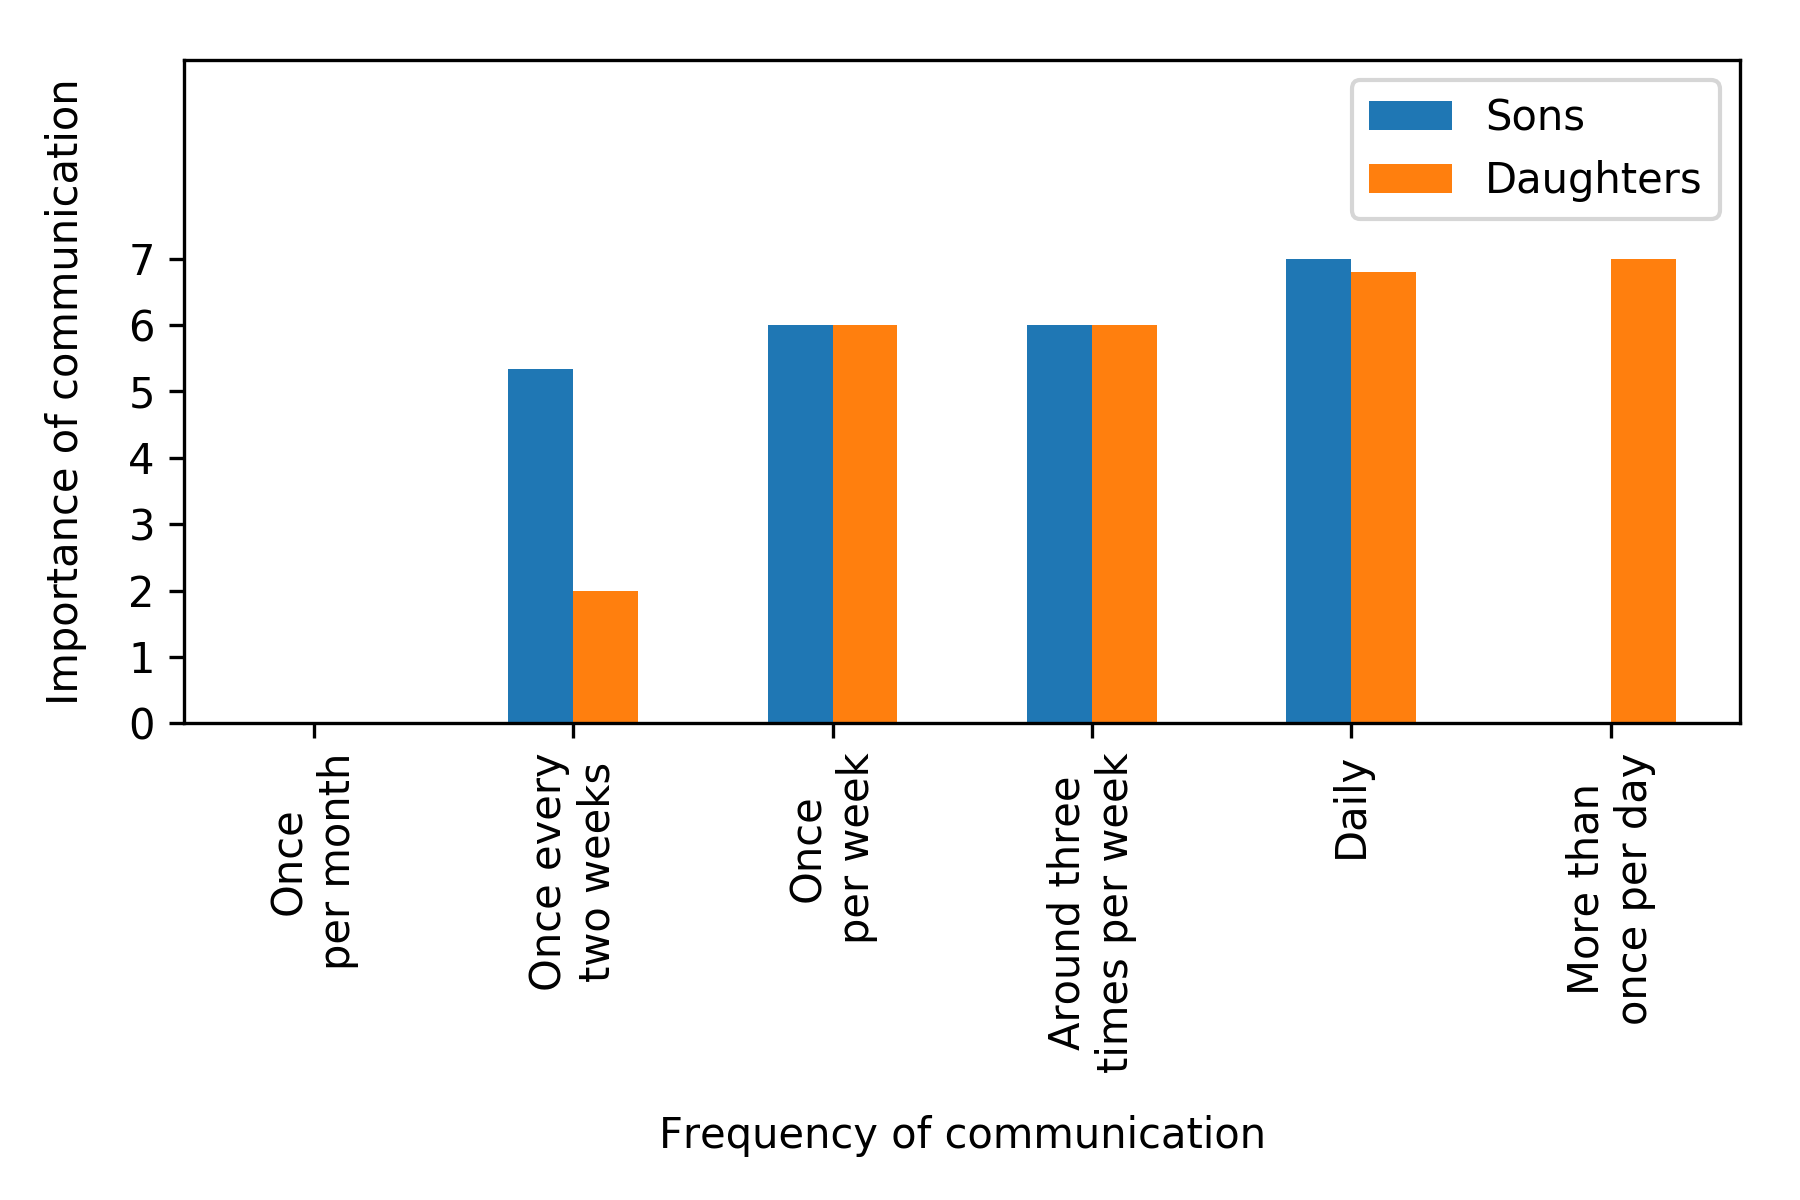
\includegraphics[scale=0.58]{plots/plot_9.png}
\end{figure}

In conclusion of this in-depth analysis around the data collected, some interesting trends have been identified. We have first reminded ourself how important each result always need to be considered in the correct context due to differences in social and cultural factors between our population and others. The analysis conclusion is based on the population sampled in the reference "western country" of Switzerland and will require more hypothesis to extend it to other social contexts (China). In fact, as we mentioned in the literature review, it is important for us to always be cautious and do not forget how different cultures determines different family "arrangements" that might give an unexpected result to trivial questionings. 
First of all, our test population proved how communication with distant family members thou ICTs is generally ranked extremely high. This result has been verified for both parent and children perspective on the issue. A second, previously not considered, result has been drawn from the data analyzed in this section regarding the \textit{gender bias} of children facing the situation. With the help of numerous and different plots it has been possible to identify such trend throughout the data. Lastly, it has been possible to test that such bias for gender is not prominent from the parent point of view, meaning that we either need to collect more data to see undiscovered patterns or indeed the importance is not determined differently for either daughters or boys. However in both cases, such hypothetical pattern along will the others illustrated previously will be discussed against the Chinese context in the coming section in order to reconnect our research findings to the LBCs issue we began with.
 
\subsection{Transposability}
\label{transposability}

Include here the interview with Mr. Antoine Kernen and % even if the interview with Mr. Kernen does not happen
discuss how results might change if the same survey was sent out to distant parents in China

%Show how important the communication technologies could be in China as well, depending on age & gender of the LBCs, duration of distant parenting

\subsection{Interview protocol}
\label{interview-protocol}

Include an explanation of the needs to have an interview protocol and explain that it has even been validated by Mrs Preissmann, expert in cognitive-experimental psychology

%What's coming next